\documentclass[12pt]{report}
\usepackage[a4paper]{geometry}
\usepackage[myheadings]{fullpage}
\usepackage{fancyhdr}
\usepackage{lastpage}
\usepackage{graphicx, wrapfig, subcaption, setspace, booktabs}
\usepackage[T1]{fontenc}
\usepackage[font=small, labelfont=bf]{caption}
\usepackage{fourier}
\usepackage[protrusion=true, expansion=true]{microtype}
\usepackage[english]{babel}
\usepackage{sectsty}
\usepackage{url, lipsum}


\newcommand{\HRule}[1]{\rule{\linewidth}{#1}}
\onehalfspacing

%-------------------------------------------------------------------------------
% HEADER & FOOTER
%-------------------------------------------------------------------------------
\pagestyle{fancy}
\fancyhf{}
\setlength\headheight{15pt}
\fancyhead[L]{DDD}
\fancyhead[R]{College of Engineering,Trivandrum}
\fancyfoot[R]{Page \thepage\ of \pageref{LastPage}}
%-------------------------------------------------------------------------------
% TITLE PAGE
%-------------------------------------------------------------------------------
\begin{document}

\title{ \normalsize \textsc{Department of Computer Science}
		\\ [2.0cm]
		\HRule{0.5pt} \\
		\LARGE \textbf{\uppercase{Detailed Design Document}}
		\HRule{2pt} \\ [0.5cm]
		\textbf{Malayalam Character Recognition }\\
		\normalsize \today \vspace*{5\baselineskip}}

\date{}

\author{
		Aarya R Shankar \\ 
		Amrith M \\
		Anand R \\
		Sarathchandran S \\ \\
		\textbf{Source: }https://github.com/amrithm98/Malayalam-Character-Recognition/
}
\maketitle
\newpage

%-------------------------------------------------------------------------------
% Section title formatting
\sectionfont{\scshape}
%-------------------------------------------------------------------------------

%-------------------------------------------------------------------------------
% BODY
%-------------------------------------------------------------------------------

\section*{Introduction}
The aim of the project is to create an character recognition system for Malayalam language. Character recognition systems have been developed for many other languages and is used in various applications. Tesseract is an OCR system implemented for English language. We think it is high time that Malayalam has one too.

In this project, we will create a classifier that classifies Malayalam alphabets using Convolutional Neural Networks. Malayalam Language has 51 letters primarily. These 51 letters are not enough for a character recognition system for this language as various symbols and their combinations are used commonly. Thus, we create a system with 133 classes which includes all the symbols that appear in the language. 

%-------------------------------------------------------------------------------
% REFERENCES
%-------------------------------------------------------------------------------
\section*{High Level Entities}
The project requires a large set of images of individual Malayalam characters. Multiple images of each character is collected and a deep learning model is trained with the help of the available dataset. We rely on neural networks for this. With the availability of huge computational capability, deep learning has proven its strength in diverse domains. We design a convolutional neural network model to train on the dataset and then fine tune the hyperparameters of the model based on the validation accuracy. From formatting the images to building the model and saving the weights of the network, the entire process happens in python. 

\section*{Low Level Entities}
\subsection*{Dataset Collection and Preparation}
The dataset of 133 Malayalam characters were collected from SPACE (Society for Promotion of Alternative Computing and Employment). It contained varying quantity of images belonging to each Malayalam character and in varying dimensions. To develop a model, the image data should have uniformity in the number of color channels and in the size of the training image. We converted all the images into grayscale and their size to 32x32 pixels. 

\subsection*{Preparing the model}
An initial convolutional Neural Network model is designed to work with the current dataset. A Convolutional Neural Network (CNN) has the following  layers: convolutional layers, pooling layers, and fully connected layers. CNNs use variation of multilayer perceptrons designed to require minimal preprocessing. They are also known as shift invariant or space invariant artificial neural networks. Convolutional layers apply a convolution operation to the input, passing the result to the next layer. Convolutional networks may include local or global pooling layers, which combine the outputs of neuron clusters at one layer into a single neuron in the next layer. This is done for downsampling a feature map obtained as the output of a convolutional layer. The final fully connected layers connects every neuron in the previous layer to the next layer. So the final downsampled feature map is stretched into a single vector and is given as input to the fully connected layer. The output of the final fully connected layer contains the required number of classes.

\begin{figure}[h]
    \centering
    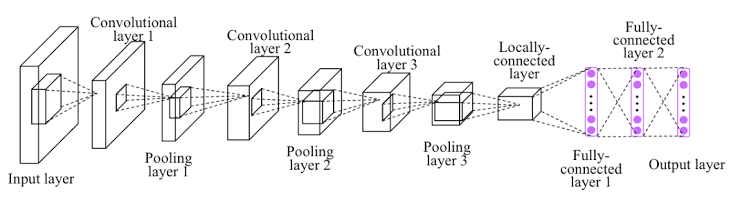
\includegraphics[width=\textwidth]{cnn.png}
    \caption{Convolutional Neural Network}
\end{figure}

\subsection*{Estimating the performance}
The weights of the the above designed model are saved and the model is tested against a validation set. The validation set is usually a separate partition of the dataset which is not used for training. To improve the accuracy, the hyperparameters such as learning rate are tweaked. If the performance does not improve, the architecture will be tweaked as well. Once the model is found to show decent accuracy, the weights can be saved and used for character classification. 

\section*{Implementation}
\subsection*{Tools Used}
\begin{itemize}
\item Python
\item Keras - Deep Learning Library in Python
\item Opencv - Computer Vision Library
\item Jupyter Notebook - IPython Notebookassociated
\end{itemize}
\subsection*{Dataset Preparation}
We got a dataset of Malayalam characters containing 133 sub folders. There were 34575 images in total. We use python libraries os and glob to do the file handling part. We give the main folder as input in our first python notebook, and initialize trainX and trainY to None. We iterate through each subfolder and picks all the .png images under each subfolder. We preprocess all these images using opencv. The preprocessing done includes resizing, converting to grayscale, and adaptive thresholding. All the images are treated as numpy arrays. After preprocessing each image, they're added to the trainX list and the corresponding labels are added to trainY list. After this, trainX and trainY are written into .npy files and saved for reuse. 

\begin{figure}[h]
    \centering
    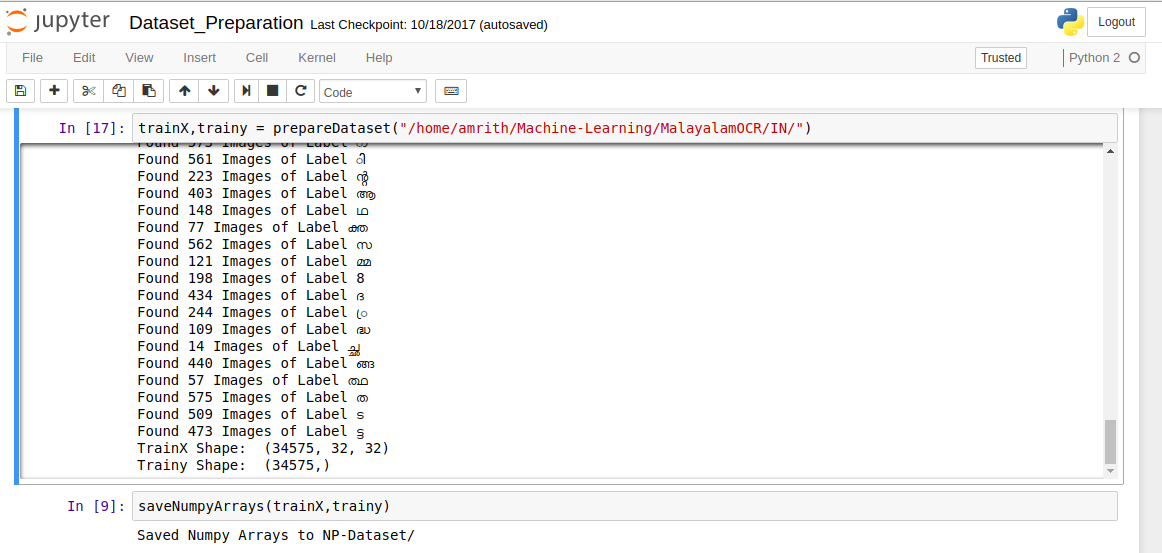
\includegraphics[width=\textwidth]{fig2.png}
    \caption{Result of preprocessing data}
\end{figure}

\subsection*{Preparing input to CNN}
We need to convert our preprocessed data into a format that CNN supports. We are using keras for deep learning. We need the input to be of (number of images, height of image, width of image, number of channels) format. Before reshaping the image we do some data cleaning. We split our data into train and test sets. This is a recommended practice in machine learning. We split our data into train and test sets in 80:20 ratio using stratified shuffle split method in sklearn library. This methods splits the existing list by randomly choosing images. We have trainX, trainY, trainY, testX and testY matrices from now on. Now we add one hot encode our labels. One hot encoding is a process by which categorical variables are converted into a form that could be provided to ML algorithms to do a better job in prediction. Here all the labels are vectors of size 133 and we set the value at index corresponding to the correct label to be 1. Now we normalize our dataset. After this we reshape all our input matrices into required format. 
 

\begin{figure}[h]
    \centering
    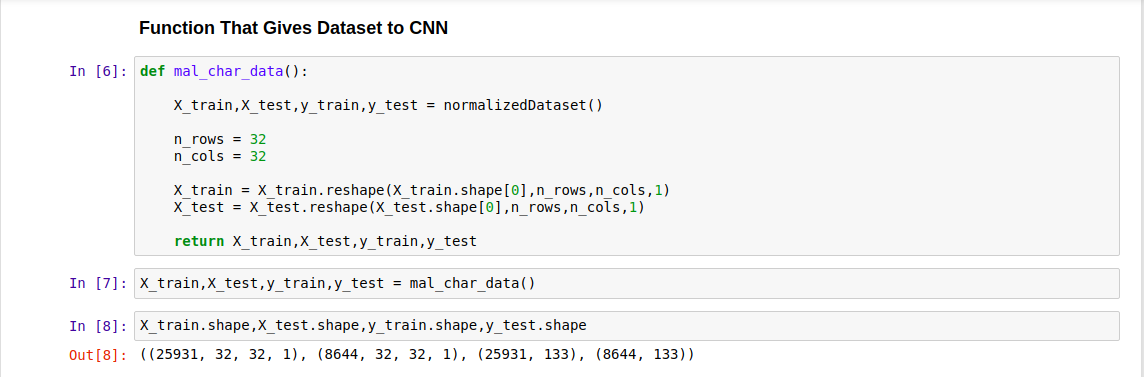
\includegraphics[width=\textwidth,height=8cm]{fig3.png}
    \caption{Preparing the inputs}
\end{figure}

\clearpage
\subsection*{Defining the architecture}
 We create the CNN model here. The created model is stored as a keras model object. Our CNN architecture has the following elements.(See Fig 4)

We stack the following layers 
\begin{itemize}
\item Convolution  - 32 3X3 kernels with RELU Activation
Zero Padding	
\item Convolution -  64 3X3 kernels with RELU Activation
\item Max Pooling - Pooling Layer 
\item Zero Padding

\item Convolution - 64 3X3 kernels with RELU Activation
\item Zero Padding
\item Convolution - 64 3X3 kernels with RELU Activation
\item Max Pooling - Pooling Layer 

\item Fully Connected Layer 1 - 2018 Neurons (Fully connected network)
\item Fully Connected Layer 2 - 512 Neurons (Fully connected network)

\item Output Layer - Output layer with 133 neurons (Softmax Activation) 
\end{itemize}
We create this model and return from within a function. Next task if training the model and training part is essentially reducing the loss. We use the cross-entropy loss(softmax loss) and optimize the loss function with a variant of gradient descent called the stochastic gradient descent. 

\begin{figure}
    \centering
    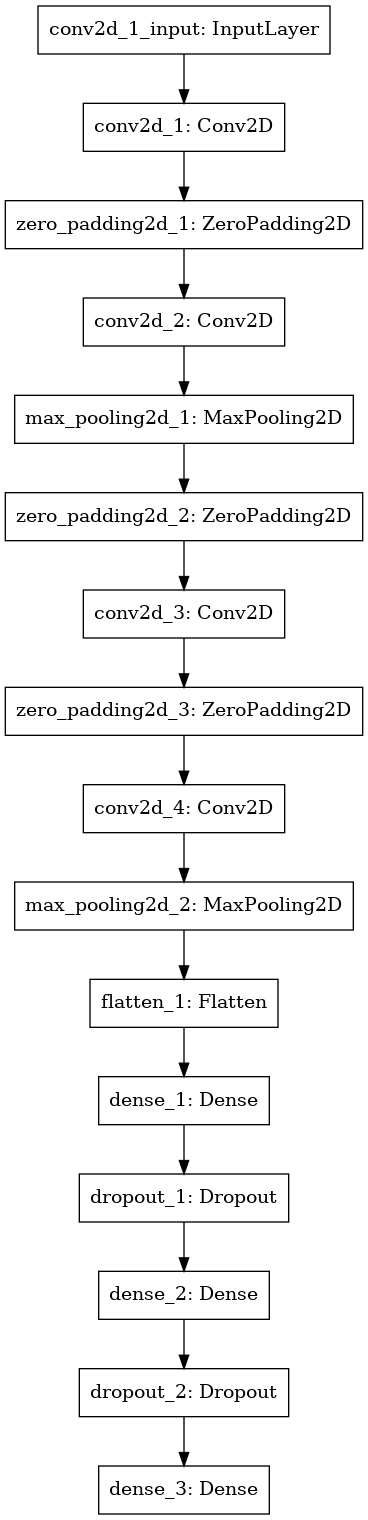
\includegraphics[scale = 0.4]{fig4.png}
    \caption{Model}
\end{figure}
\newpage

\subsection*{Optimizer}
We use stochastic gradient descent method to reduce the loss. Stochastic gradient descent (SGD) performs a parameter update for each training example x(i)and label y(i):(See Fig 5)

\begin{figure}[h]
    \centering
    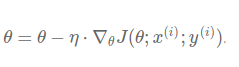
\includegraphics{eqn1.png}
    \caption{SGD Update}
\end{figure}

Batch gradient descent performs redundant computations for large datasets, as it recomputes gradients for similar examples before each parameter update. SGD does away with this redundancy by performing one update at a time. It is therefore usually much faster and can also be used to learn online. 
SGD performs frequent updates with a high variance that cause the objective function to fluctuate heavily as in image.(See Fig 6)

\begin{figure}[h]
    \centering
    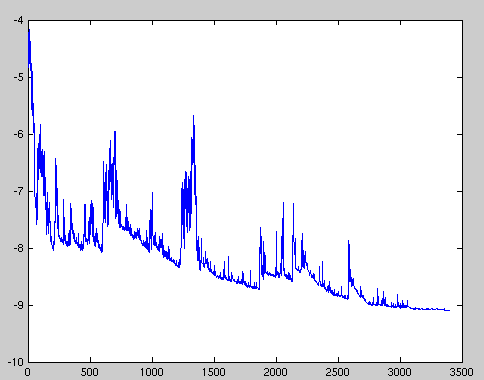
\includegraphics[scale=.5]{fig5.png}
    \caption{Stochastic gradient descent}
\end{figure}

While batch gradient descent converges to the minimum of the basin the parameters are placed in, SGD's fluctuation, on the one hand, enables it to jump to new and potentially better local minima. On the other hand, this ultimately complicates convergence to the exact minimum, as SGD will keep overshooting. However, it has been shown that when we slowly decrease the learning rate, SGD shows the same convergence behaviour as batch gradient descent, almost certainly converging to a local or the global minimum for non-convex and convex optimization respectively. 
Its code fragment simply adds a loop over the training examples and evaluates the gradient w.r.t. each example. Note that we shuffle the training data at every epoch as explained.(See Fig 7)

\begin{figure}[h]
    \centering
    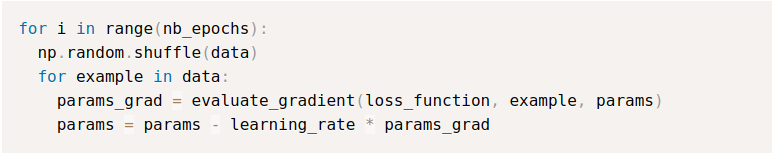
\includegraphics[width=\textwidth]{sgd.png}
    \caption{Stochastic gradient descent Implementation}
\end{figure}

\subsection*{Loss Function - Softmax (Cross Entropy Loss)
}
The softmax function squashes the outputs of each unit to be between 0 and 1, just like a sigmoid function. But it also divides each output such that the total sum of the outputs is equal to 1 (check it on the figure above).
The output of the softmax function is equivalent to a categorical probability distribution, it tells you the probability that any of the classes are true.
Mathematically the softmax function is shown below, where z is a vector of the inputs to the output layer (if you have 10 output units, then there are 10 elements in z). And again, j indexes the output units, so j = 1, 2, ..., K.

\begin{figure}[h]
    \centering
    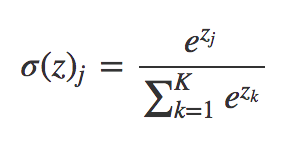
\includegraphics[scale=.5]{eqn2.png}
    \caption{Softmax Loss Function}
\end{figure}

\subsection*{ReLU Activation Function}

ReLU. The Rectified Linear Unit has become very popular in the last few years. It computes the function f(x)=max(0,x)f(x)=max(0,x). In other words, the activation is simply thresholded at zero (see image above on the left). There are several pros and cons to using the ReLUs:

\begin{itemize}

\item (+) It was found to greatly accelerate (e.g. a factor of 6 in Krizhevsky et al.) the convergence of stochastic gradient descent compared to the sigmoid/tanh functions. It is argued that this is due to its linear, non-saturating form.
\item (+) Compared to tanh/sigmoid neurons that involve expensive operations (exponentials, etc.), the ReLU can be implemented by simply thresholding a matrix of activations at zero.
\item (-) Unfortunately, ReLU units can be fragile during training and can "die". For example, a large gradient flowing through a ReLU neuron could cause the weights to update in such a way that the neuron will never activate on any datapoint again. If this happens, then the gradient flowing through the unit will forever be zero from that point on. That is, the ReLU units can irreversibly die during training since they can get knocked off the data manifold. For example, you may find that as much as 40\% of your network can be "dead" (i.e. neurons that never activate across the entire training dataset) if the learning rate is set too high. With a proper setting of the learning rate this is less frequently an issue.

\end{itemize}

\subsection*{Training Optimizations}
\subsubsection*{Drop out}
Dropout layers provide a simple way to avoid overfitting. This is the regularization technique we use in this model. We give dropout with 50\% probability in the last fully connected layers which cancels 50\% of the activations randomly to the next layer. This helps the model to learn multiple representations of data.

\begin{figure}[h]
    \centering
    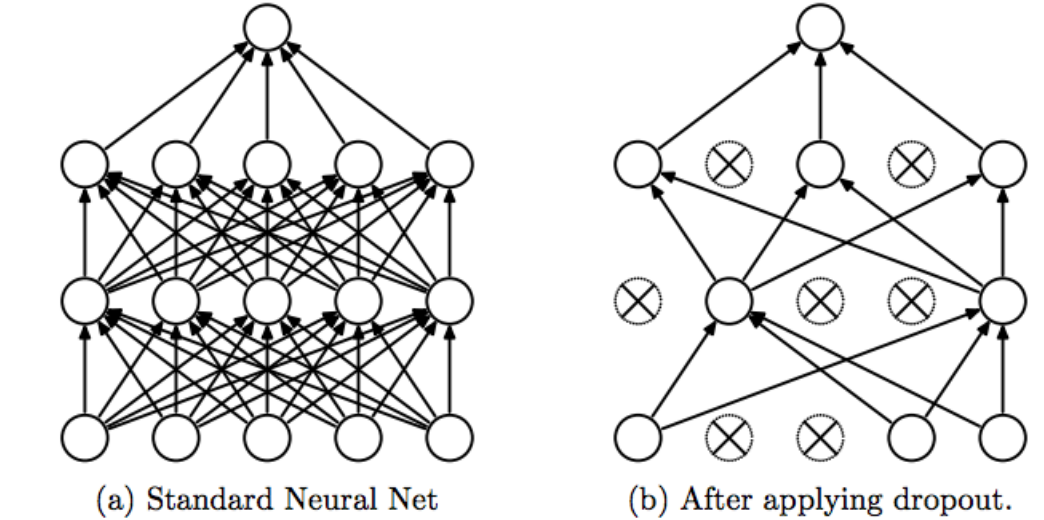
\includegraphics[scale=.25]{dropout.png}
    \caption{Dropout}
\end{figure}

\newpage
\subsection*{Training Phase}
The Training phase was completed with the help of floydhub deep learning service (floydhub.com). We took a free account and started another GPU enabled jupyter-notebook. From the notebook, we downloaded the dataset and used all the preprocessing functions we created to get the input ready. Once the input was ready, we used the keras fit() method to start the training . The initial hyper parameters did not give good results and we stopped the training with very high loss.

The second training had number of epochs set to 20 and learning rate to 0.001. We happened to get a training accuracy of 97.11 on the training set. We added batch normalization to the existing model and retrained it to get a test set accuracy of 98. 69\%. 
The following were the parameters used for training: 

\begin{itemize}

\item batch\_size = 256
\item epochs = 20
\item learning\_rate = 0.001
\item decay = $ 10^{-6} $
\item momentum = .9

\end{itemize}

Momentum technique was used in SGD. After the training was completed , weights were saved into .h5 files. This is the result of the training and we use this weights for making predictions on images. 

\begin{figure}[h]
    \centering
    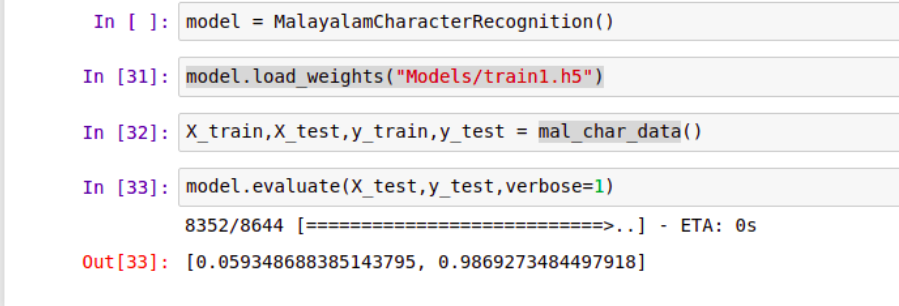
\includegraphics[width=\textwidth]{result.png}
    \caption{Loss \& Accuracy on Test Set}
\end{figure}

\clearpage
\subsection*{Predictions}
We created another notebook for testing the predictions. We loaded our model with the weights we trained and predicted the test image labels. We took out some random images in the test set and predicted the labels. The result were very accurate but the limitation is that the model can only recognize one specific font.

Few results of the predictions are here :

The labels are seen on the top left of the image. 

\begin{figure}[h]
    \centering
    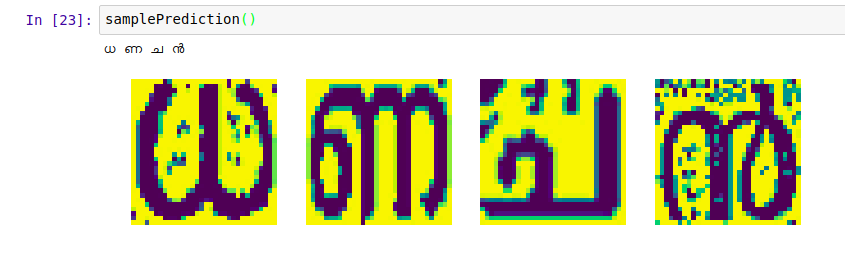
\includegraphics[width=\textwidth]{samp1.png}
    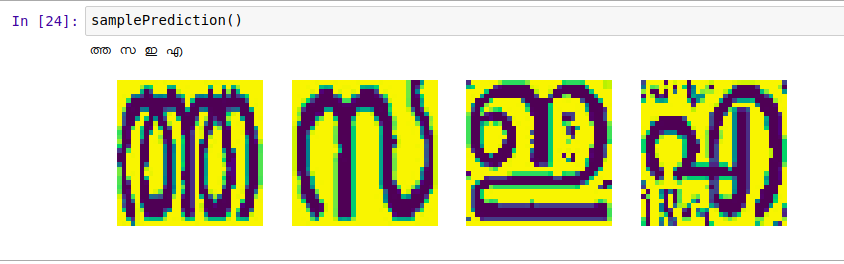
\includegraphics[width=\textwidth]{samp2.png}
    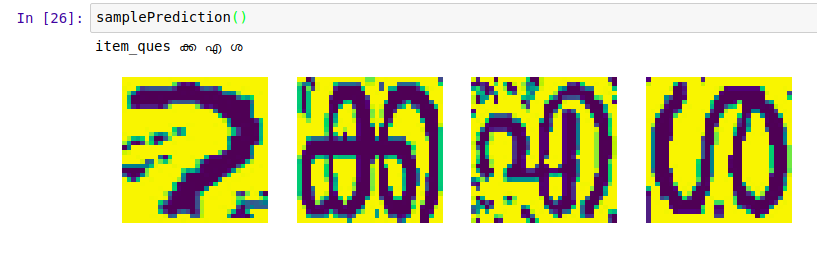
\includegraphics[width=\textwidth]{samp3.png}
    \caption{Sample Images From Test Set}
\end{figure}

% \begin{figure}[h]
%     \centering
%     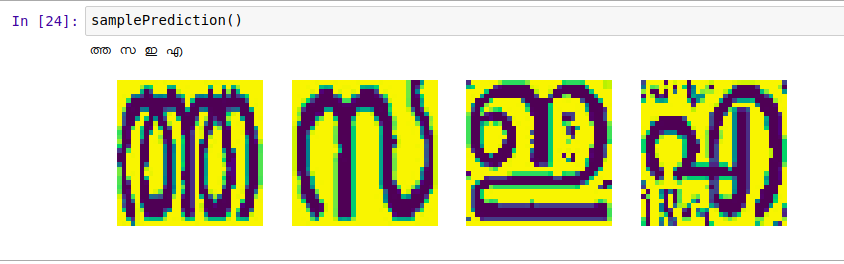
\includegraphics[width=\textwidth]{samp2.png}
%     \caption{sample2}
% \end{figure}

% \begin{figure}[h]
%     \centering
%     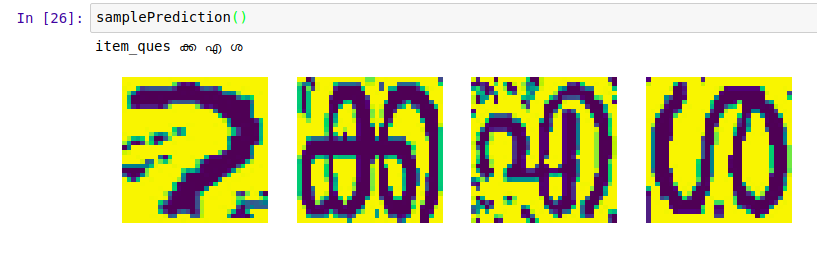
\includegraphics[width=\textwidth]{samp3.png}
%     \caption{sample3}
% \end{figure}

\clearpage
\subsection*{Deployment}
We implemented a python script which predicts the image label on inputting an alphabet. The script initially loads the model and the weights and has a menu driven interface which allows users to input the images. Labels are predicted and shown as soon as the images are inputted.  

\begin{figure}[h]
    \centering
    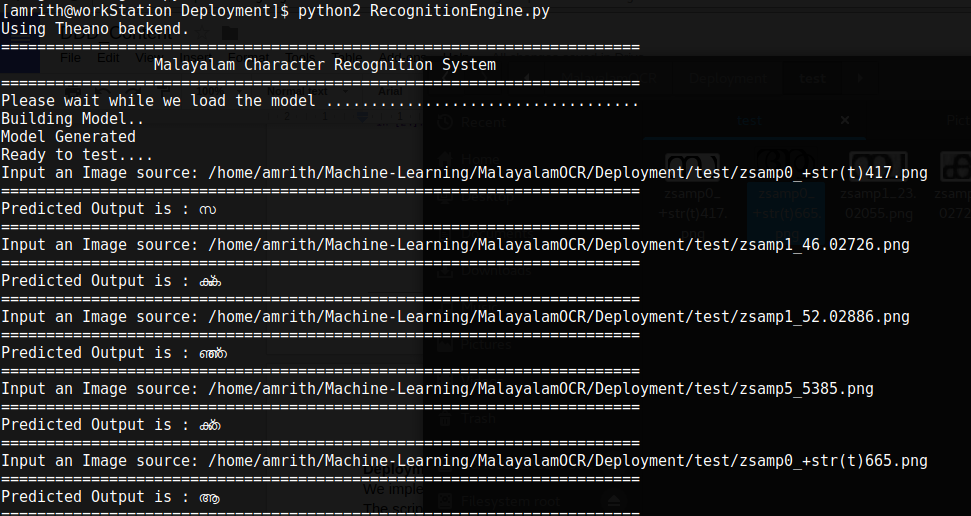
\includegraphics[scale = .5]{deployment.png}
    \caption{Python Script Predicting Labels}
\end{figure}

\newpage
\section*{Class Diagram}
This is the class diagram for the entire project. The project does not contain a class , so we assume that the entire project is a class and the core data structures are the attributes of the class. The functions that operate on this method acts as the class methods.
\begin{figure}[h]
    \centering
    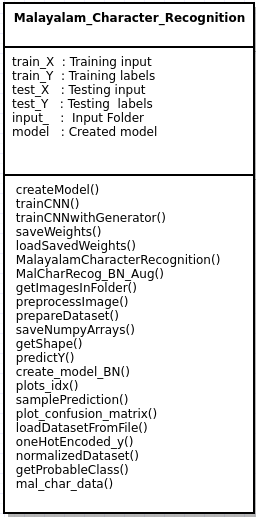
\includegraphics[scale = 1 ]{classdia.png}
    \caption{Class Diagram for the entire project}
\end{figure}

\clearpage
\section*{Benefits}
\begin{itemize}
\item First and foremost, we can use this to develop an OCR for sample2Malayalam language.


\item Our Kerala Government has enlisted Malayalam as the language of all official documents. Hence, a malayalam OCR is necessary for digitalising them efficiently. Our model can speed up its development process by a considerable factor.
\item This project may be modified to read the malayalam scripts and process them using NLP (Natural Language Processing) and use a text-to-speech software as an aid to blind people.
\end{itemize}

\section*{Risks}
\begin{itemize}
\item The biggest problem in developing a model is that if the dataset is not good enough, the model will not be good enough. Hence the dataset to be prepared must have the various characters and their combinations.
\item Training a large set of dataset needs a very efficient GPU, which is not easily available.

\end{itemize}

\section*{Literature Review}


 In this review, we'll be focusing on previous papers written on Malayalam character recognition. 

Intitial attempt for Malayalam character recognition had been done by Space Kerala. This project used support vector machines to classify Malayalam characters. They used to split an image into 8 pieces and then analyse the shape of each portion. After obtaining the class scores of all the eight portions, then used to correlate the probability of each portion the correct class score and make a prediction. Another paper on the same topic was written by few professors at CUSAT in which they implemented character recognition system using chain code histogram method. 
A chain code histogram counts the frequency of occurrence of each of the 8 directions. This means the information of the order of occurrence of the directions is lost. However, instead of storing the entire chain code, this enables storing only 8 data values.
The loss of accuracy is negligible. The storage space gained is immensely useful for embedded systems which have constrained resources. Coming to Convolutional Neural networks,they are extremely flexible in the types of data they can support. Neural Networks do a decent job at learning the important features from basically any data structure, without having to manually derive features. Deep Learning is about learning increasingly more abstract representations in a layer-wise manner. Each layer feeds from the layer below and then sends the output to the layer above and so on. This process leads to neurons high up the hierarchy being sensitive to particular complete objects or scenes in case of vision applications that is.CNNs are designed to work with image data, while SVM is a more generic classifier.CNNs extract features while SVM simply maps its input to some high dimensional space where (hopefully) the differences between the classes can be revealed.CNNs are deep architectures while SVMs are shallow.



\section*{Conclusion}


 Considering all the entities, benefits and the risks of this project, we can conclude that our project is a probable one and will also be a beneficial one to the society.



\section*{References}
\begin{itemize}
\item Offline handwritten Malayalam Character Recognition based on chain code histogram (Jomy John,KV Pramod,Kannan Balakrishnan)
\item Lekha OCR - SPACE Kerala
\item Srivastava, Nitish, et al. "Dropout: a simple way to prevent neural networks from overfitting." Journal of Machine Learning Research 15.1 (2014): 1929-1958.
\item Stochastic gradient descent methods for estimation with large data sets (Dustin Tran, Panos Toulis, Edoardo M. Airoldi)
\item Sutskever, Ilya, et al. "On the importance of initialization and momentum in deep learning." ICML (3) 28 (2013): 1139-1147.
\item Krizhevsky, Alex, Ilya Sutskever, and Geoffrey E. Hinton. "Imagenet classification with deep convolutional neural networks." Advances in neural information processing systems. 2012.
\item Ioffe, Sergey, and Christian Szegedy. "Batch normalization: Accelerating deep network training by reducing internal covariate shift." arXiv preprint arXiv:1502.03167 (2015). 

\end{itemize}



\end{document}



